\documentclass[10pt,a4paper]{article}

\usepackage[T1]{fontenc}
\usepackage[utf8]{inputenc}
\usepackage{lmodern}
\usepackage{geometry}
\usepackage{hyperref}
\usepackage{microtype}
\usepackage{graphicx}
\usepackage{amsmath}
\usepackage{tabularx}
\usepackage{array}
\usepackage{longtable}

\geometry{margin=2.5cm}
\setlength{\emergencystretch}{2em}
\newcolumntype{L}[1]{>{\raggedright\arraybackslash}p{#1}}
\newcolumntype{Y}{>{\raggedright\arraybackslash}X}
\hypersetup{
  colorlinks=true,
  linkcolor=black,
  citecolor=black,
  urlcolor=blue,
  pdftitle={ImpactLLM Observatory: An Open Observatory for the Environmental Footprint of LLMs},
  pdfauthor={Arnault Pachot and Thierry Petit}
}

\title{ImpactLLM Observatory:\\An Open Observatory for the Environmental Footprint of LLMs}
\author{Arnault Pachot \and Thierry Petit}
\date{March 14, 2026}

\begin{document}

\maketitle

\begin{abstract}
The environmental literature on large language models (LLMs) is growing, but the evidence remains difficult to reuse because values are dispersed across papers, model cards, reports, and dashboards with heterogeneous units and system boundaries. We present \emph{ImpactLLM}, an open observatory and screening tool for exploring the environmental footprint of current LLMs. The contribution is intentionally practical rather than grand-theoretical. First, the project provides a source-linked evidence layer that can be reused through a tabular dataset, a local API, an MCP server, and a public web interface. Second, it offers a rapid application-level estimator driven by natural-language descriptions rather than by long technical forms. The current release combines an inference-only application estimator with multi-factor screening views for both inference and training. In both cases, the project starts from observed literature anchors, then applies bounded multi-factor proxies that remain explicit and inspectable. In a domain where direct telemetry is usually unavailable for the most-used proprietary models, we argue that an open, auditable observatory is itself a useful scientific contribution.
\end{abstract}

\textbf{Keywords:} LLMs, open data, environmental footprint, inference, screening method, API.

\section{Introduction}
Environmental evaluation of LLMs is now discussed across several analytical levels: model training, prompt-level inference, service delivery, water use, hardware lifecycle, and data-center electricity demand \cite{strubell2019,rillig2023,luccioni2023,ren2024,morrison2025,elsworth2025,li2025water,iea2025}. Yet the practical bottleneck is no longer simply the absence of quantified values. The literature now contains many values, but they are difficult to compare, audit, and reuse because they differ in unit of analysis, system boundary, geography, and traceability.

This paper addresses that bottleneck with a narrower claim than many AI-impact papers. \emph{ImpactLLM} is not presented as a precision measurement system for proprietary LLM services, and it does not claim to discover a universal law linking parameter counts to energy use. Its contribution is instead twofold.

First, it provides an open observatory of environmental indicators for current LLMs. The observatory exposes source-linked records, model metadata, bibliographic references, and comparative views that remain inspectable by users. Second, it provides a rapid screening tool for application-level inference assessment. The user can describe an LLM-enabled application in natural language; the system extracts a compact scenario and returns an inference-focused estimate together with its assumptions, sources, and calculation details. This ``fast estimate from natural language'' design is deliberate: in many practical settings, users do not know dozens of technical serving parameters, but they can describe their application, model, country, and usage volume.

This positioning reflects a practical methodological judgment. The current AI market is dominated by a small number of hosted LLM services such as ChatGPT, Claude, Gemini, and Copilot, precisely the systems for which direct environmental telemetry is the least accessible. Yet the absence of direct measurement does not prevent strong claims from circulating. On the contrary, the public debate is now saturated with contradictory assertions, rough extrapolations, and decontextualized figures. In this context, the relevant choice is not between perfect measurement and approximation. For dominant proprietary services, perfect measurement is usually unavailable. The practical choice is therefore between opaque, unverifiable claims and a transparent, source-linked, auditable approximation framework. \emph{ImpactLLM} adopts the second position.

This gap is especially visible for proprietary LLMs. While some product-level figures and a few industrial anchors have recently become public, model-level environmental values for proprietary systems are still rarely published with enough methodological detail to support direct comparison or reuse. The most widely used systems are often the least transparent: the serving hardware, routing logic, batching behavior, architecture, and deployment geography needed for direct environmental attribution generally remain undisclosed.

The scientific claim of the paper is therefore modest but useful. In a field dominated either by low-level telemetry tools or by opaque provider-side information, an open, reusable observatory coupled with an explicit screening estimator can fill an important operational gap.

\section{State of the Art}
The current landscape can be grouped into four broad methodological families.

The first family consists of hardware-instrumented experiment- or run-level trackers. These tools estimate energy or carbon from machine-level telemetry and retained electricity factors. Early experiment-level accounting in NLP is exemplified by Strubell et al. \cite{strubell2019}. Current open-source tools such as \emph{CarbonTracker} \cite{anthony2020carbontracker} and \emph{CodeCarbon} \cite{codecarbon2026} operationalize this logic for machine-learning workloads. They are useful when the evaluator controls the hardware, but not for proprietary hosted LLM APIs.

The second family consists of instrumented serving benchmarks. Here the objective is to measure standardized inference workloads on explicit serving stacks. Elsworth et al. provide an important production anchor by reporting prompt-level energy for Gemini Apps \cite{elsworth2025}. The recent \emph{ML.ENERGY Benchmark} extends this benchmark logic to automated inference-energy measurement and optimization \cite{mlenergy2025}. These approaches are more relevant to LLM inference than generic run trackers, but they remain tightly tied to the measured serving context.

The third family consists of bottom-up estimators for opaque or partially opaque hosted services. In this family, the evaluator does not observe provider-side telemetry directly. Instead, the estimate is reconstructed from proxies such as token volume, model class, architecture assumptions, likely hardware, and geography. \emph{EcoLogits} is the clearest operational example of this family for current hosted LLM services \cite{ecologits2026}. \emph{ImpactLLM} belongs to the same family, with a stronger emphasis on source-linked evidence and explicit methodological inspection.

The fourth family consists of cloud- or infrastructure-level accounting tools such as \emph{Cloud Carbon Footprint} \cite{cloudcarbonfootprint2026} and provider dashboards from AWS, Microsoft, Google Cloud, and OVHcloud \cite{awsccft2026,azureeid2026,gcloudcarbon2026,ovhtracker2024}. These tools are valuable for infrastructure governance, but they do not directly yield the footprint of one proprietary LLM request without an additional attribution layer.

Two broader lessons follow from the literature. First, the footprint of LLMs is multi-dimensional and should not be collapsed into one number \cite{rillig2023,li2025water,morrison2025}. Second, unit of analysis and system boundary matter as much as the numerical value itself \cite{ren2024}. The missing piece is therefore a reusable evidence layer that preserves this heterogeneity instead of hiding it.

\section{Contribution and Data Layer}
\emph{ImpactLLM Observatory} is organized around one core design principle: one reusable quantified value per record, with its source and comparability context. The current release contains 76 records spanning 11 core sources and four analytical phases: training, inference, infrastructure, and lifecycle. This iteration also expands the market-model catalog to 41 entries, adding legacy Grok (1/2) and Claude 2 releases plus a curated set of GPT-era models such as Megatron-Turing NLG, Jurassic-1, Gopher, GLaM, LaMDA, and OPT to the previously tracked OpenAI and Mistral families. All inference and training columns were recomputed so the observatory data reflect those additional models and the most recent parameter inputs. Each record stores at least a unique identifier, citation, year, analytical phase, impact category, metric name, value, unit, model or scope, geography, data type, source locator, source URL, and free-text note.

This structure separates three dimensions that are often conflated in narrative reviews: the observed phenomenon, the method used to produce the number, and the scope to which the number applies. It also supports a second metadata layer describing comparability-oriented fields such as unit of analysis, source type, uncertainty level, and applicability domain.

The same evidence base is exposed through four reuse layers: a tabular dataset, a local HTTP API, an MCP server, and a bilingual public web observatory \cite{impactllmrepo2026}. The scientific point is not that each interface is novel on its own, but that they all reuse the same source-linked evidence base. This makes the web observatory, the programmatic interfaces, and the paper mutually auditable rather than loosely aligned artifacts.

This observatory angle matters because, to our knowledge, openly accessible infrastructures that jointly provide (i) source-level environmental indicators for LLMs, (ii) comparative views of current models, and (iii) an application-oriented inference screening interface remain rare. Existing tools often provide either instrumentation, or estimation, or datasets, but not all three within one openly inspectable workflow.


\noindent The screening proxies themselves are described in full in the companion paper \emph{Transparent Screening for LLM Inference and Training Impacts}; the remainder of this article focuses on the resulting observatory outputs.


\section{Illustrative Results}
The public observatory standardizes model comparison under one hour of active use corresponding to 1,000 input tokens, 550 output tokens, one LLM request per interaction, and approximately 34.6 interactions per hour, derived from a reading-speed convention \cite{brysbaert2019}. The underlying dataset and derived tables were refreshed for the March 2026 release, so the published values mirror the recalculated inference and training columns for the expanded market-model catalog. This provides a common comparison space before application-specific annualization.

Table \ref{tab:short-results} summarizes a few illustrative outputs. The first block shows how the standardized observatory makes model orders of magnitude legible. The second block shows how the same proxy can be annualized at the software-feature level from compact, natural-language scenarios.

\begin{table}[htbp]
\centering
\small
\begin{tabularx}{\textwidth}{|L{4.0cm}|L{2.5cm}|L{2.2cm}|Y|}
\hline
Case & Energy & Carbon & Interpretation \\
\hline
Ministral 3B, one active hour & 0.19 Wh & 0.0077 gCO$_2$e & Small hybrid model under a French provider-country proxy \\
\hline
GPT-5 mini, one active hour & 5.90 Wh & 2.272 gCO$_2$e & Medium proprietary hosted model under a US provider-country proxy \\
\hline
Claude Opus 4.1, one active hour & 103.53 Wh & 39.860 gCO$_2$e & Very large proprietary estimate illustrating the steep growth of screening orders of magnitude \\
\hline
Support chatbot, Ministral 8B, 20{,}000 conversations/month & 2.38 kWh/year & 96 gCO$_2$e/year & Low-carbon annual result despite high usage because the retained electricity factor is favorable \\
\hline
Retrieval assistant, GPT-5 mini, 4{,}000 uses/month & 12.31 kWh/year & 4.74 kgCO$_2$e/year & Higher annualized result driven by hosted-service assumptions and US electricity contextualization \\
\hline
\end{tabularx}
\caption{Illustrative outputs from the current observatory and application estimator. These values are screening estimates, not audited declarations.}
\label{tab:short-results}
\end{table}

These examples illustrate three practical properties of the method. First, annualization matters: apparently small unit values become relevant when multiplied by real usage. Second, the chosen model profile matters materially. Third, the retained electricity mix can dominate the carbon interpretation, which is why country contextualization is explicitly shown in the interface. Just as importantly, these results can be obtained quickly from natural-language inputs while keeping the extracted scenario and assumptions visible in the interface.

\subsection{Observatory Visualizations}
Figure \ref{fig:inference-release} follows the release sequence of OpenAI, Claude, Grok, and Mistral models against the project’s inference carbon estimate, keeping the vertical axis logarithmic to hold small and large models together. Figure \ref{fig:training-release} applies the same structure to the retained direct training CO$_2$e estimates, which are even more dispersed.

\begin{figure}[htbp]
\centering
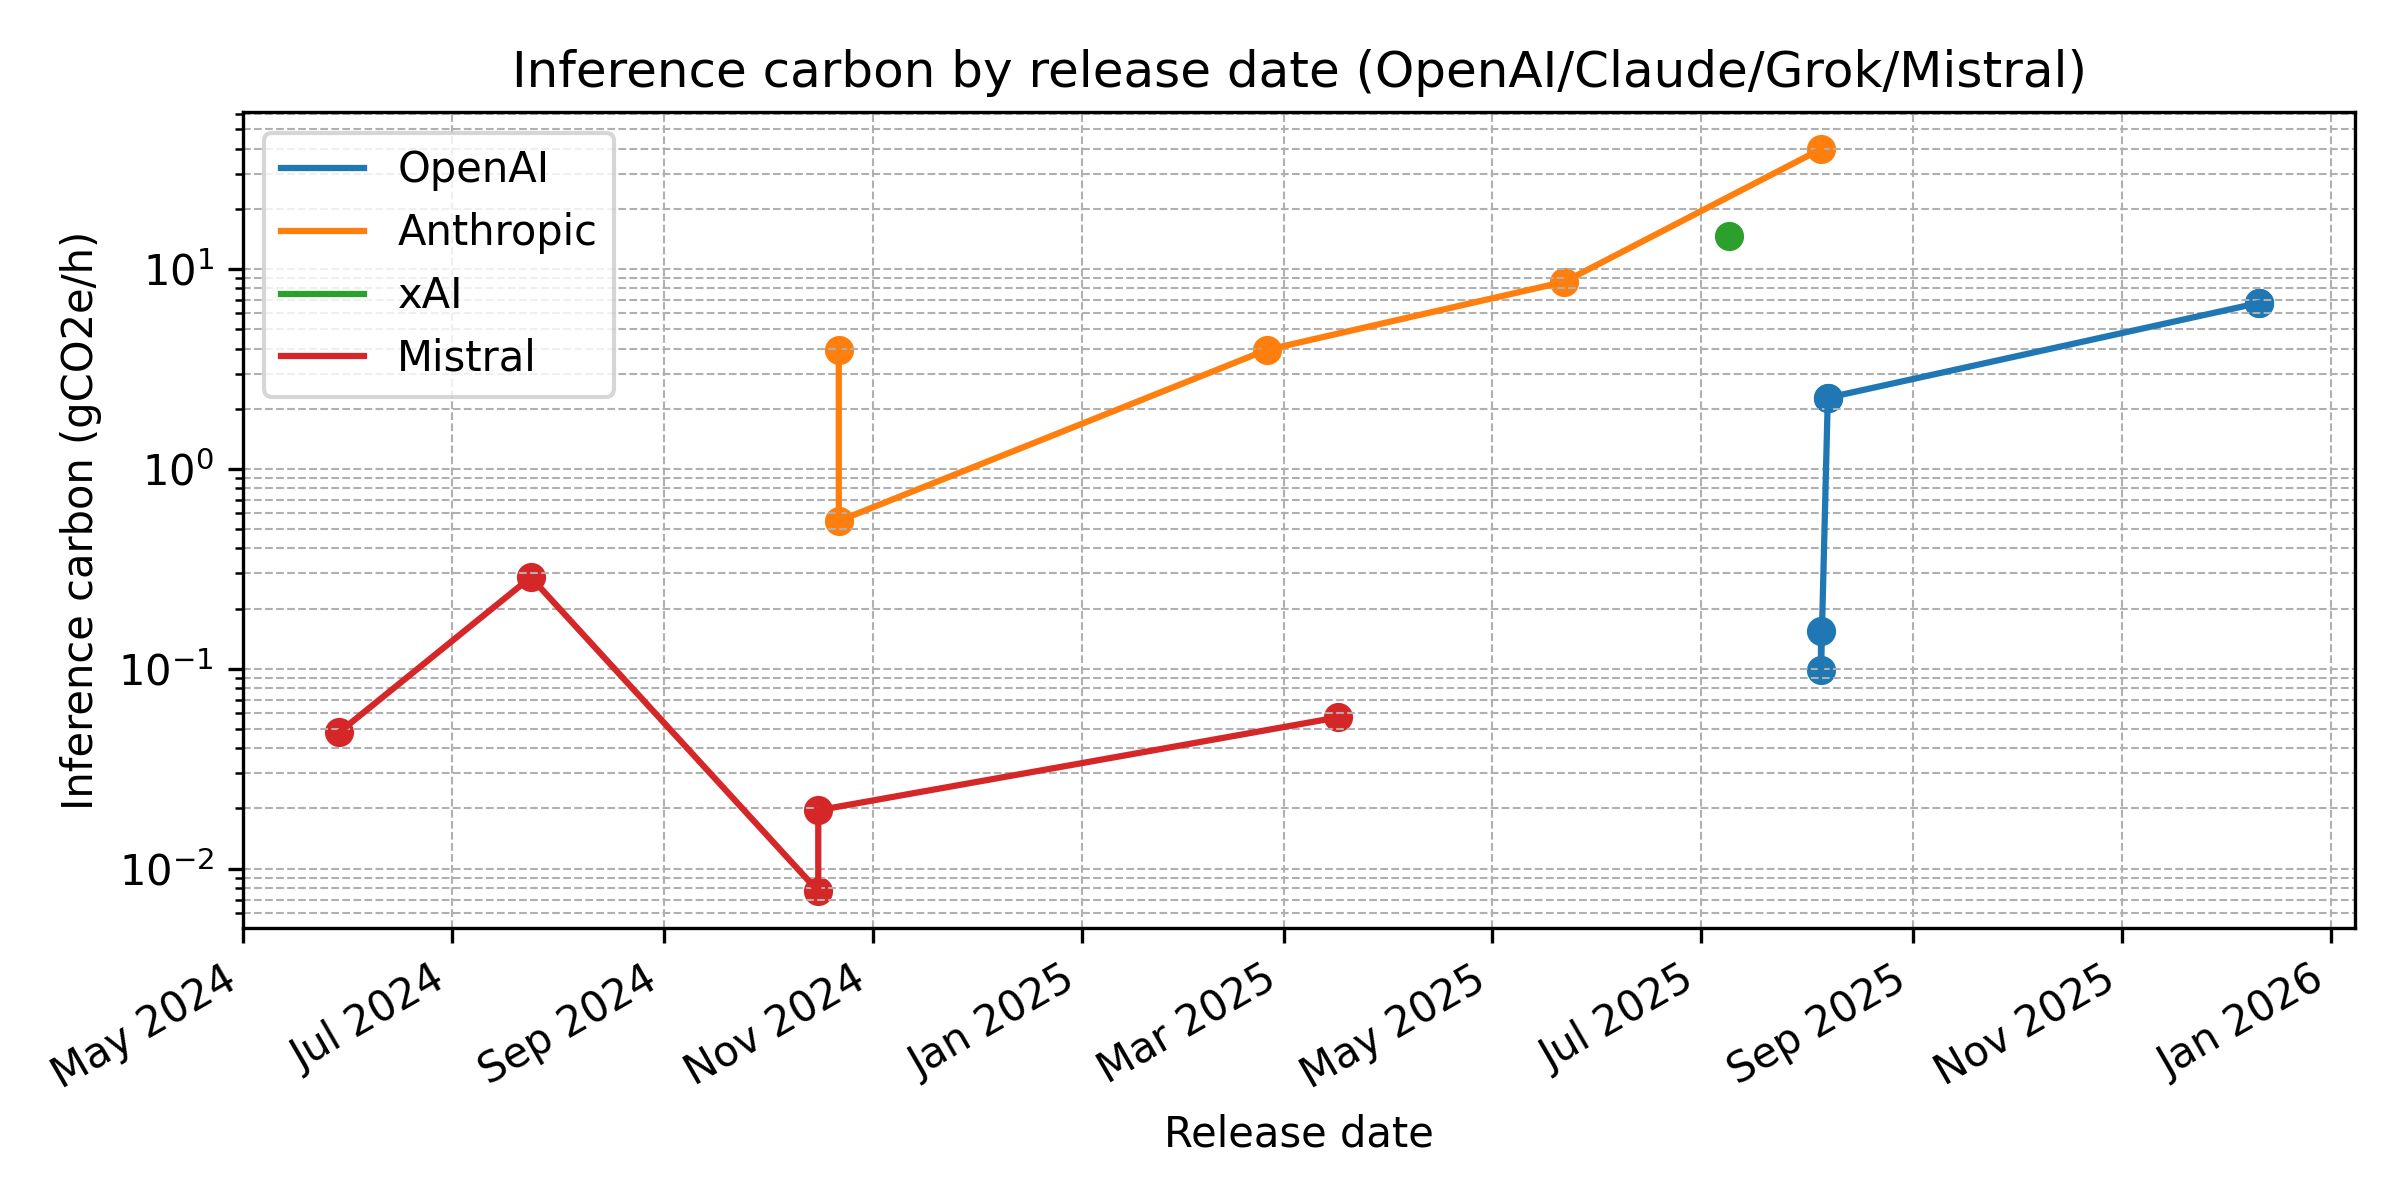
\includegraphics[width=0.85\linewidth]{figures/inference_release_timeline.png}
\caption{Inference carbon (gCO$_2$e/h) for the OpenAI, Anthropic, xAI, and Mistral families, plotted against each model’s release month. The logarithmic scale keeps the large orders of magnitude accessible.}
\label{fig:inference-release}
\end{figure}

\begin{figure}[htbp]
\centering
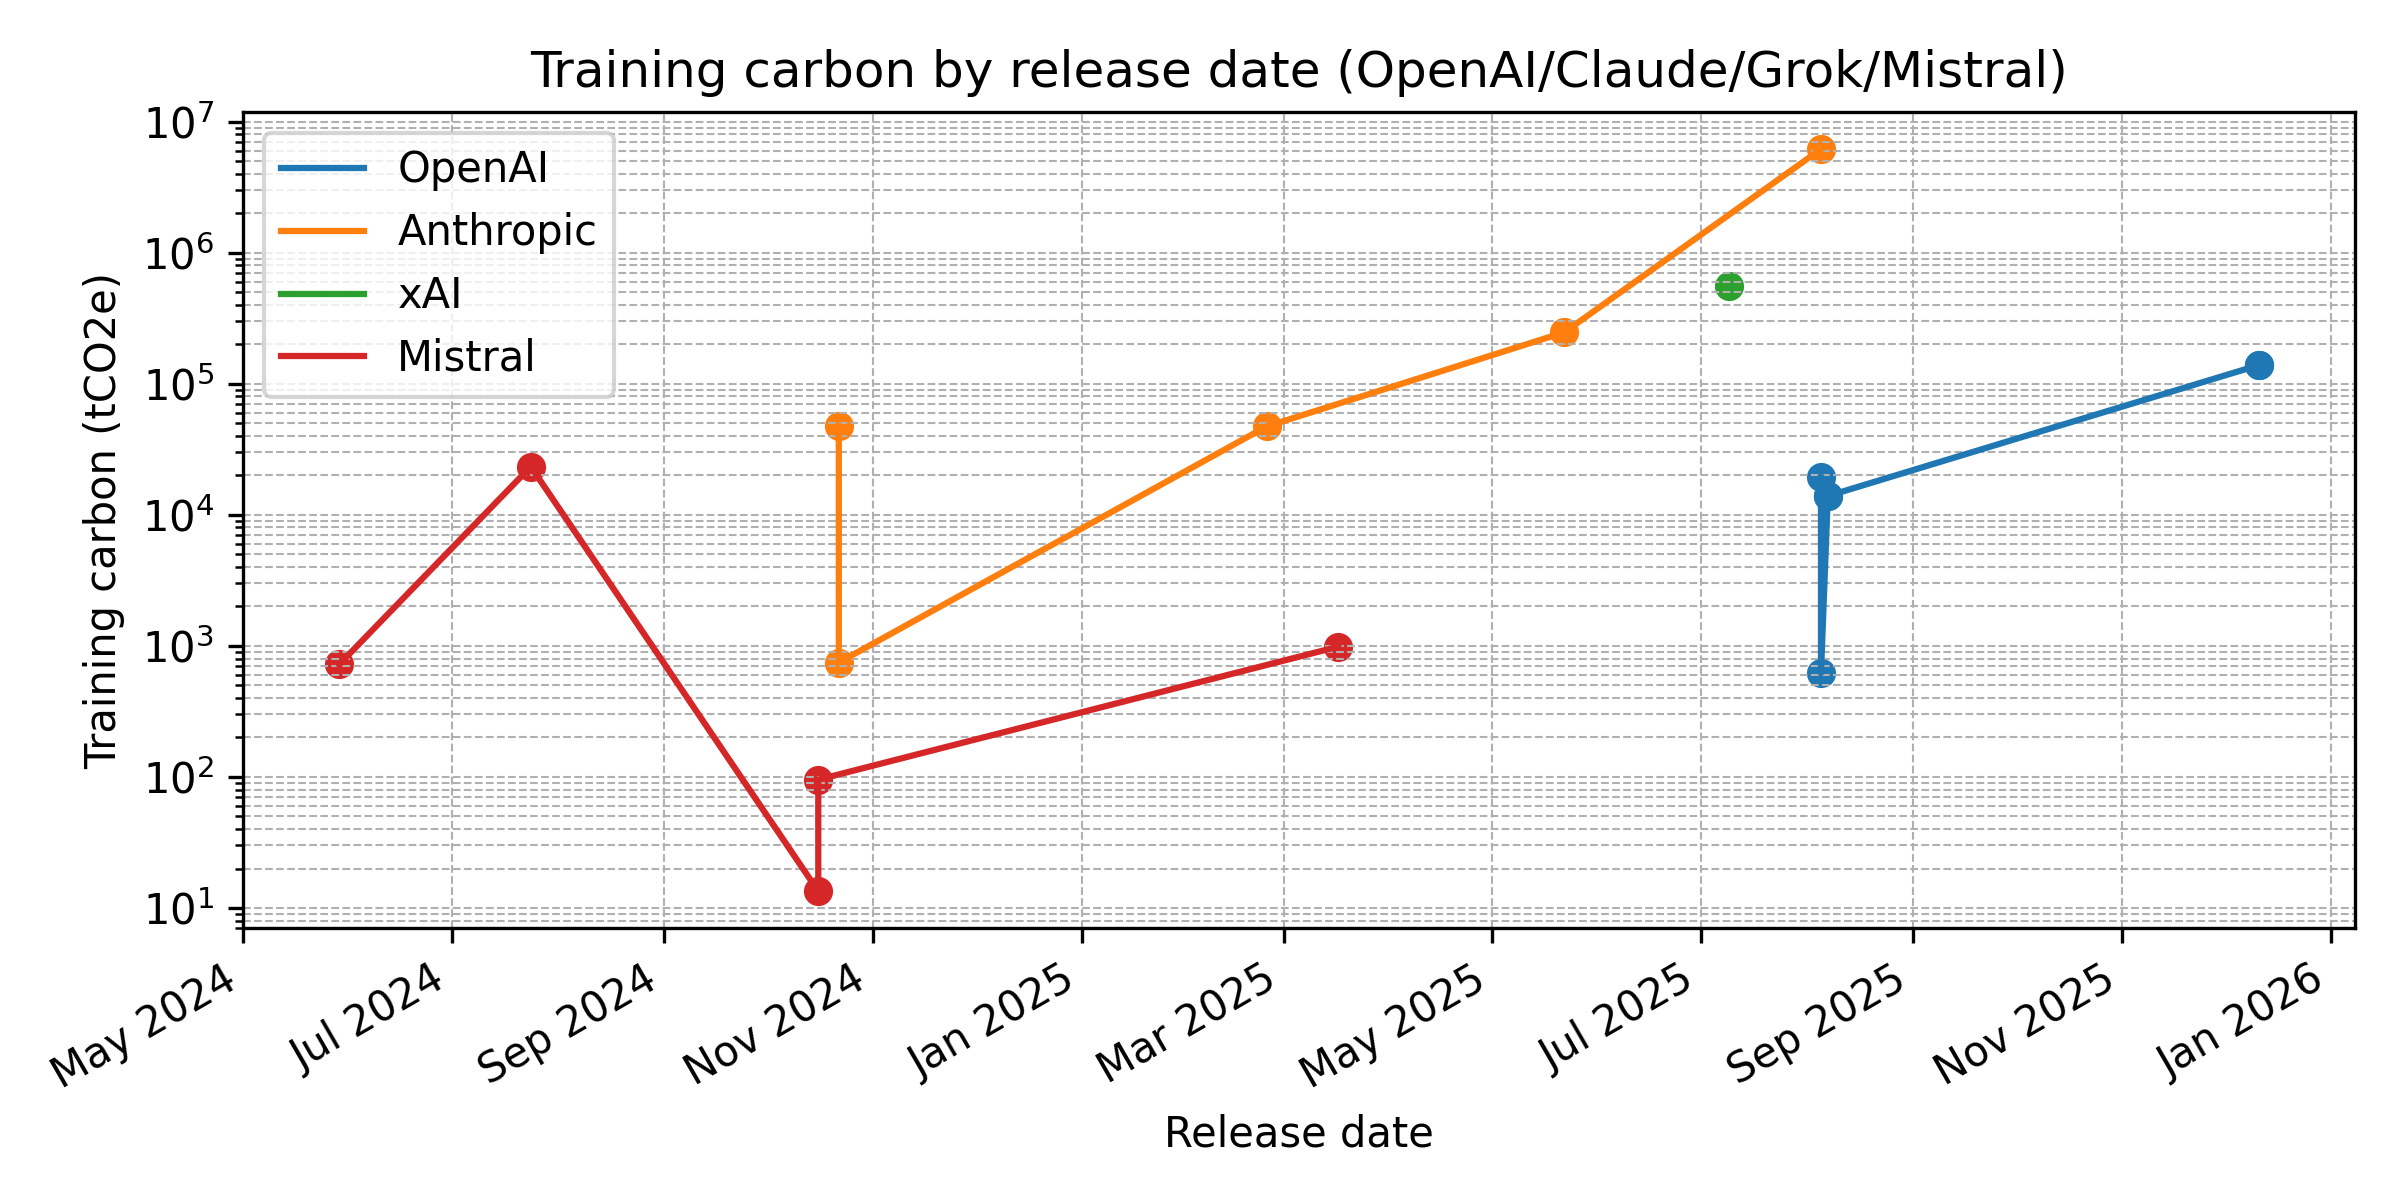
\includegraphics[width=0.85\linewidth]{figures/training_release_timeline.png}
\caption{Direct training CO$_2$e (tCO$_2$e) from the same release sequence. The timeline emphasizes how training estimates scatter across multiple magnitudes even within the same provider families.}
\label{fig:training-release}
\end{figure}

For completeness, Table \ref{tab:catalog-results} reports the current calculated values for all 41 market models tracked in the March 2026 release. The purpose of this table is documentary: it makes the observatory outputs directly inspectable in the paper, while the web interface remains the primary medium for interactive exploration.

\begin{longtable}{|L{4.0cm}|L{2.0cm}|L{2.2cm}|L{1.7cm}|L{1.8cm}|}
\caption{Calculated environmental indicators for the 41 market models currently tracked by ImpactLLM. Inference values correspond to the standardized one-hour scenario used in the observatory. Training values are multi-factor screening estimates.}\label{tab:catalog-results}\\
\hline
Model & Inference Wh/h & Inference gCO$_2$e/h & Training GWh & Training ktCO$_2$e \\
\hline
\endfirsthead
\hline
Model & Inference Wh/h & Inference gCO$_2$e/h & Training GWh & Training ktCO$_2$e \\
\hline
\endhead
\hline
GPT-5.2 & 17.59 & 6.77 & 155.26 & 138.75 \\
\hline
GPT-5.2-pro & 17.59 & 6.77 & 155.26 & 138.75 \\
\hline
GPT-5 mini & 5.90 & 2.27 & 15.57 & 13.91 \\
\hline
GPT-5 nano & 5.90 & 2.27 & 15.57 & 13.91 \\
\hline
GPT-OSS 120B & 0.40 & 0.15 & 21.56 & 19.27 \\
\hline
GPT-OSS 20B & 0.26 & 0.10 & 0.69 & 0.62 \\
\hline
Claude Opus 4.1 & 103.53 & 39.86 & 6900.35 & 6166.82 \\
\hline
Claude Sonnet 4 & 22.44 & 8.64 & 276.01 & 246.67 \\
\hline
Claude 3.5 Sonnet & 10.23 & 3.94 & 52.83 & 47.21 \\
\hline
Claude 3.7 Sonnet & 10.23 & 3.94 & 52.83 & 47.21 \\
\hline
Claude 3.5 Haiku & 1.43 & 0.55 & 0.83 & 0.75 \\
\hline
Gemini 2.5 Pro & 12.46 & 4.80 & 69.00 & 61.67 \\
\hline
Gemini 2.5 Flash & 5.22 & 2.01 & 11.04 & 9.87 \\
\hline
Gemini 2.5 Flash-Lite & 2.06 & 0.79 & 1.55 & 1.39 \\
\hline
Gemini 2.0 Flash & 2.06 & 0.79 & 1.55 & 1.39 \\
\hline
Grok 4 & 38.04 & 14.65 & 621.03 & 555.01 \\
\hline
Llama 3.1 8B & 0.46 & 0.18 & 0.11 & 0.10 \\
\hline
Llama 3.1 70B & 3.61 & 1.39 & 8.58 & 7.66 \\
\hline
Llama 3.1 405B & 19.13 & 7.37 & 287.06 & 256.54 \\
\hline
Ministral 3B & 0.19 & 0.01 & 0.02 & 0.01 \\
\hline
Ministral 8B & 0.49 & 0.02 & 0.11 & 0.10 \\
\hline
Mistral Large & 7.18 & 0.29 & 26.10 & 23.32 \\
\hline
Mistral Small 3.1 24B & 1.43 & 0.06 & 1.10 & 0.99 \\
\hline
Codestral 22B & 1.20 & 0.05 & 0.81 & 0.72 \\
\hline
Qwen2.5 7B & 0.41 & 0.22 & 0.09 & 0.08 \\
\hline
Qwen2.5 32B & 1.72 & 0.93 & 1.79 & 1.60 \\
\hline
Qwen2.5 72B & 3.71 & 2.00 & 9.07 & 8.11 \\
\hline
DeepSeek V3 & 2.76 & 1.49 & 675.40 & 603.60 \\
\hline
DeepSeek R1 & 2.89 & 1.56 & 675.40 & 603.60 \\
\hline
\end{longtable}

\section{Limitations}
The main limitation is epistemic rather than computational. For proprietary hosted models, the evaluator does not observe the real serving stack, hardware, batch behavior, or data-center geography directly. The method therefore remains a proxy-informed estimate, not a direct measurement. The bounded interval is intended to make that limitation visible rather than to eliminate it.

A second limitation is anchor sparsity. Prompt-level inference anchors remain scarce, and the method currently relies heavily on Elsworth et al. for the main operational prompt-energy anchor \cite{elsworth2025}. Training anchors are also sparse and require additional priors on training tokens, regime, architecture, and hardware class. More published request-level and training-level benchmarks would improve both calibration and uncertainty framing.

A third limitation concerns scope. The current user-facing estimate is still inference-only. Training, embodied hardware impacts, software-system overheads, and water contextualization remain documented in the evidence base, and training is now screened in the observatory, but these dimensions are not yet integrated into the personalized application estimate.

A fourth limitation concerns natural-language scenario extraction. The ``fast estimate'' workflow improves usability, but it also introduces interpretation assumptions when users provide incomplete descriptions. For that reason, the extracted scenario, assumptions, and retained defaults are systematically displayed alongside the result.

\section{Conclusion}
\emph{ImpactLLM} proposes a different kind of contribution to the LLM-environment literature. Its main novelty is not a new physical model, but an open, source-linked infrastructure that makes environmental evidence reusable across a dataset, an API, an MCP server, and a public observatory. On top of that evidence layer, the project implements a transparent inference-only screening method for current LLM services, including proprietary ones, and a rapid interface that starts from natural-language descriptions rather than long technical forms.

The value of the project lies precisely in this combination of restraint and reuse. It does not claim hidden provider telemetry, and it does not collapse heterogeneous evidence into a single opaque score. Instead, it publishes the records, the assumptions, the interfaces, and the extrapolative method together. In a field where the difficulty is increasingly one of comparability, accessibility, and traceability rather than raw numerical absence, an open observatory plus a fast screening workflow is a legitimate scientific contribution in its own right \cite{impactllmrepo2026}.

This is the sense in which the project should be read. For the most widely used hosted LLMs, direct environmental measurement is usually not publicly available, while public and policy discussions nevertheless continue to rely on numerical claims. In such a setting, doing nothing does not preserve rigor; it leaves the field open to opaque, inconsistent, and non-reproducible assertions. \emph{ImpactLLM Observatory} therefore argues for a more disciplined middle ground: not false precision, but explicit approximation; not hidden assumptions, but auditable proxies; not definitive measurement, but a reusable framework that can be challenged, updated, and improved as better evidence becomes available.

\bibliographystyle{plain}
\bibliography{references_ImpactLLM}

\end{document}
